%%%%%%%%%%%%%%%%%%%%%%%%%%%%%%%%%%%%%%%%%%%%%%%%%%%%%%%%%%%%%%%%%%%%%%%%%%%%%%%%
%% Plantilla de memoria en LaTeX para TFG/TFM - Universidad Rey Juan Carlos
%%
%% Por Gregorio Robles <grex arroba gsyc.urjc.es>
%%     Felipe Ortega   <felipe.ortega@urjc.es>
%%     Grupo de Sistemas y Comunicaciones (GSyC)
%%     Escuela Técnica Superior de Ingenieros de Telecomunicación
%%     Universidad Rey Juan Carlos
%%
%% (Muchas ideas tomadas de Internet, colegas del GSyC, antiguos alumnos...
%%  etc. Muchas gracias a todos)
%%
%% La última versión de esta plantilla está siempre disponible en:
%%     https://github.com/glimmerphoenix/plantilla-memoria
%%
%% - Ejecución en sistema local:
%% Para obtener el documento en PDF, ejecuta en la shell:
%%   make
%%
%% A diferencia de la anterior versión, que usaba la herramienta pdfLaTeX 
%% para compilar el documento, esta nueva versión de la plantilla usa
%% XeLaTeX. Es un compilador más moderno que, entre otras mejoras, incluye
%% soporte nativo para caracteres con codificación UTF-8, traducción políglota
%% de referencias (usando Biblatex) y soporte para fuentes OTF. Esta última
%% característic permite, por ejemplo, insertar iconos de la colección 
%% Fontawesome en el texto.
%%
%% XeLaTeX viene ya incluido en todas las distribuciones modernas de LaTeX.
%%
%% - Edición y ejecución en línea: 
%% Puedes descargar y subir la plantilla a
%% Overleaf, un editor de LaTeX colaborativo en línea. Overleaf ya tiene
%% instalados todos los paquetes LaTeX y otras dependencias software para
%% que esta plantilla compile correctamente.
%%
%% IMPORTANTE: Si compilas este documento en Overleaf, recuerda cambiar
%% la configuración (botón "Menu" en la esquina superior izquierda de la interfaz)
%% y elegir la opción Compiler --> XeLaTeX. En caso contrario no funcionará.
%%
%% - Nota: las imágenes deben ir en PNG, JPG, EPS o PDF. También se pueden usar
%% imágenes en otros formatos con algunos cambios en el preámbulo del documento.

%%%%%%%%%%%%%%%%%%%%%%%%%%%%%%%%%%%%%%%%%%%%%%%%%%%%%%%%%%%%%%%%%%%%%%%%%%%%%%%%

\documentclass[a4paper, 12pt]{book}

%%-- Geometría principal (dejar activada la siguiente línea en la versión final)
\usepackage[a4paper, left=2.5cm, right=2.5cm, top=3cm, bottom=3cm]{geometry}
%%-- Activar esta línea y comentar la anterior en modo borrador, para comentarios al margen
%\usepackage[a4paper, left=2.5cm, right=2.5cm, top=3cm, bottom=3cm, marginparwidth=60pt]{geometry}

%%-- Hay que cargarlo antes que las traducciones
\usepackage{listing}                    % Listados de código

% Traducciones en XeLaTeX
\usepackage{polyglossia}
\setmainlanguage{spanish}    % Comenta esta línea si tu memoria es en inglés

% Traducciones particulares para español
% Caption tablas
\gappto\captionsspanish{
	\def\tablename{Tabla}
	\def\listingscaption{Código}
	\def\refname{Bibliografía}
	\def\appendixname{Apéndice}
	\def\listtablename{Índice de tablas}
	\def\listingname{Código}
	\def\listlistingname{Índice de fragmentos de código}
}

%% Tipografía y estilos
\usepackage[OT1]{fontenc}               % Keeps eulervm happy about accents encoding

% Símbolos y fuentes matemáticas elegantes: Euler virtual math fonts
% ¡Importante! Carga siempre las fuentes math AMS Euler ANTES QUE fontspec
\usepackage{amsmath}
\usepackage{amssymb}
\usepackage[OT1,euler-digits,euler-hat-accent,small]{eulervm}

% En XeLaTeX las fuentes se especifican con fontspec
\usepackage{fontspec}
\defaultfontfeatures{Scale=MatchLowercase, Ligatures=TeX}     % Default option in font config

% Fix para fuentes usadas con operadores y \mathrm
\DeclareSymbolFont{operators}{\encodingdefault}{\familydefault}{m}{n}

% Configura la fuente principal (serif): MinionPro
\setmainfont[Scale=0.96]{TeX Gyre Pagella}
% Configura la fuente sans-serif (\sffamily)
\setsansfont[Scale=MatchLowercase]{Lato}
% Configura la fuente para letra monoespaciada: Source Code Pro, escala 0.85
\setmonofont[Scale=0.85]{Source Code Pro}

%%-- Familias de fuentes específicas
%%-- Se pueden definir etiquetas para familias de fuentes personalizadas
%%-- que luego puedes emplear para cambiar el formato de una parte de texto
%%-- Ejemplo:
% \newfontfamily{\myriadprocond}{Myriad Pro Semibold Condensed.otf}

%%-- Opciones de interlineado y espacios
\linespread{1.07}                   % Aumentar interlineado para fuentes tipo Palatino
\setlength{\parskip}{\baselineskip} % Separar párrafos con línea en blanco

%%-- Hipervínculos
\usepackage{url}

%%-- Gráficos y tablas
\PassOptionsToPackage{
    dvipdfmx,usenames,dvipsnames,
    x11names,table}{xcolor}             % Definiciones de colores
\PassOptionsToPackage{xetex}{graphicx}

\usepackage{subfig}                     % Subfiguras
\usepackage{pgf}
\usepackage{svg}                        % Integración de imágenes en formato SVG
\usepackage{float}                      % H para posicionar figuras
\usepackage{booktabs}                   % Already loads package xcolor
\usepackage{multicol}                   % multiple column layout facilities
\usepackage{colortbl}                   % For coloured tables

%%-- Bibliografía con Biblatex y Biber
% Más info:
% https://www.overleaf.com/learn/latex/Biblatex_bibliography_styles
% https://www.overleaf.com/learn/latex/biblatex_citation_styles
\usepackage[
    backend=biber,
    style=numeric,
    sorting=none
    ]{biblatex}
\addbibresource{refs.bib}
\DeclareFieldFormat{url}{\mkbibacro{URL}\addcolon\nobreakspace\url{#1}}
%\usepackage[nottoc, notlot, notlof, notindex]{tocbibind} %% Opciones de índice

%%-- Matemáticas e ingeniería
% El paquete units permite mostrar unidades correctamente
% Permite escribir unidades con espaciado y estilo de fuente correctos
\usepackage[ugly]{units}         
% Ejemplo de uso: $\unit[100]{m}$ or $\unitfrac[100]{m}{s}$
% Entornos matemáticos
\newtheorem{theorem}{Theorem}

% Paquetes adicionales
\usepackage{url}                        %% Gestión correcta de enlaces
\usepackage{float}                      %% H para posicionar figuras
\usepackage[nottoc, notlot, notlof, notindex]{tocbibind}    %% Opciones de índice
\usepackage{metalogo}                   %% Múltiples logos para XeLaTeX

% Fuentes especiales y glifos
\usepackage{ccicons}                % Creative Commons icons
\usepackage{metalogo}               % XeTeX logo
\usepackage{fontawesome5}           % Fontawesome 5 icons
\usepackage{adforn} 

% Blindtext
% Opciones pangram, bible, random (defecto)
\usepackage[pangram]{blindtext}
% Lorem ipsum
\usepackage{lipsum}
% Kant lipsum
\usepackage{kantlipsum}

\usepackage{fancyvrb}               % Entornos verbatim extendidos
	\fvset{fontsize=\normalsize}    % Tamaño de fuente por defecto en fancy-verbatim
	
% Configura listas (itemize, enumerate) con iconos personalizados
% Fácil reinicio de numeración con enumerate
% Info: http://ctan.org/pkg/enumitem
\usepackage[shortlabels]{enumitem}
% Usar \usageitem para configurar iconos personalizados en listas
\newcommand{\usageitem}[1]{%
	\item[%
	{\makebox[2em]{\strut\color{GSyCblue} #1}}%
	]
}

%%-- Definición de colores personalizados
% \definecolor{LightGrey}{HTML}{EEEEEE}
% \definecolor{darkred}{rgb}{0.5,0,0}     %% Refs. cruzadas
% \definecolor{darkgreen}{rgb}{0,0.5,0}   %% Citas bibliográficas
% \definecolor{darkblue}{rgb}{0,0,0.5}    %% Hiperenlaces ordinarios (también ToC)

%%-- Configuración fragmentos de código
%%-- Minted necesita Python Pygments instalado en el sistema para funcionar
%%-- En Overleaf ya está instalada esta dependencia
% \usepackage[center, labelfont=bf]{caption}
\usepackage{minted}

%%-- Se debe cargar aquí para evitar warnings
\usepackage{csquotes}                   % Para traducciones con biblatex

%%-- Glosario de términos
\usepackage[acronym]{glossaries}
\makeglossaries
\loadglsentries{glossary}

% % Definición de cabeceras del documento, usando fancyhdr
% \usepackage{fancyhdr}
% %% Configuración de cabeceras para el cuerpo principal del documento
% \pagestyle{fancy}
% \fancyhead{}
% \fancyhead[RO,LE]{\myriadprocond{\thepage}}
% \renewcommand{\chaptermark}[1]{\markboth{\chaptername\ \thechapter.\ #1}{}}
% \renewcommand{\sectionmark}[1]{\markright{\thesection.\ #1}}
% \fancyhead[RE]{\myriadprocond{\leftmark}}
% \fancyhead[LO]{\myriadprocond{\rightmark}}
% \renewcommand{\headrulewidth}{0pt}
% \setlength{\headheight}{15pt} %% Al menos 15pt para evitar warning al compilar
% \fancyfoot{}
% %% Configuración para páginas con cabecera en blanco
% \fancypagestyle{plain}{%
% \fancyhf{}% clear all header and footer fields
% \fancyhead[RO,LE]{\myriadprocond{\thepage}}
% \renewcommand{\headrulewidth}{0pt}%
% \renewcommand{\footrulewidth}{0pt}%
% }

%%-- Metadatos del doc
\title{Memoria del Proyecto}
\author{Nombre del autor}

%%-- Hiperenlaces, siempre se carga al final del preámbulo
\usepackage[colorlinks]{hyperref}
\hypersetup{
    pdftoolbar=true,	% Muestra barra de herramientas en Adobe Acrobat
	pdfmenubar=true,	% Muestra menú en Adobe Acrobat
	pdftitle={Título doc en ventana del visor o navegador},
	pdfauthor={Nombre del alumno/a},
	pdfcreator={ETSII/ETSIT, URJC},
	pdfproducer={XeLaTeX},
	pdfsubject={Topic1, Topic2, Topic3},
	pdfnewwindow=true,              %links open in new window
    colorlinks=true,                % false: boxed links; true: coloured links
    linkcolor=Firebrick4,           % enlaces internos 
    citecolor=Aquamarine4,          % enlaces a citas bibliográficas
    urlcolor=RoyalBlue3,            % hiperenlances ordinarios
    linktocpage=true                % Enlaces en núm. pág. en ToC
}

%%%---------------------------------------------------------------------------
% Comentarios en línea de revisión
% Este bloque se puede borrar cuando finalizamos el borrador

% \usepackage[colorinlistoftodos]{todonotes}
% \usepackage{verbatim}
%%%---------------------------------------------------------------------------

\begin{document}

%%-- Configuración común para todos los entornos listing
%%-- Descomentar para usar y personalizar valores
%\lstset{%
%breakatwhitespace=true,
% breaklines=true, 
% basicstyle=\footnotesize\ttfamily,
% keywordstyle=\color{blue},
% commentstyle=\color{green!40!black}, 
% language=Python} 
 

%%%%%%%%%%%%%%%%%%%%%%%%%%%%%%%%%%%%%%%%%%%%%%%%%%%%%%%%%%%%%%%%%%%%%%%%%%%%%%%%
% PORTADA

\begin{titlepage}
\begin{center}
\begin{tabular}[c]{c c}
%\includegraphics[bb=0 0 194 352, scale=0.25]{logo} &
\includegraphics[scale=1.5]{img/LogoURJC.png}
%&
%\begin{tabular}[b]{l}
%\Huge
%\textsf{UNIVERSIDAD} \\
%\Huge
%\textsf{REY JUAN CARLOS} \\
%\end{tabular}
\\
\end{tabular}

\vspace{3cm}

\Large 
INGENIERÍA EN TECNOLOGÍAS DE LA TELECOMUNICACIÓN 

\vspace{0.4cm}

\large
Curso Académico 2021/2022

\vspace{0.8cm}

Trabajo Fin de Grado

\vspace{2cm}

\LARGE VISUALIZACIÓN Y ANÁLISIS\\
DE DATOS 
\vspace{3cm}

\large
Autora : María Cristina Gallego Herrero \\
Tutor : Dr. Felipe Ortega 
\end{center}
\end{titlepage}

\newpage
\mbox{}
\thispagestyle{empty} % para que no se numere esta pagina


%%%%%%%%%%%%%%%%%%%%%%%%%%%%%%%%%%%%%%%%%%%%%%%%%%%%%%%%%%%%%%%%%%%%%%%%%%%%%%%%
%%%% Para firmar
\clearpage
\pagenumbering{gobble}
\chapter*{}

\vspace{-4cm}
\begin{center}
\LARGE
\textbf{Trabajo Fin de Grado/Máster}

\vspace{1cm}
\large
Título del Trabajo con Letras Capitales para Sustantivos y Adjetivos

\vspace{1cm}
\large
\textbf{Autora :} María Cristina Gallego Herrero  \\
\textbf{Tutor :} Dr. Felipe Ortega 

\end{center}

\vspace{1cm}
La defensa del presente Proyecto Fin de Grado se realiza el día 3\qquad$\;\,$ de
\qquad\qquad\qquad\qquad \newline de 20XX, siendo calificada por el siguiente tribunal:


\vspace{0.5cm}
\textbf{Presidente:}

\vspace{0.8cm}
\textbf{Secretario:}

\vspace{0.8cm}
\textbf{Vocal:}


\vspace{0.8cm}
y habiendo obtenido la siguiente calificación:

\vspace{0.8cm}
\textbf{Calificación:}


\vspace{0.8cm}
\begin{flushright}
Móstoles/Fuenlabrada, a \qquad$\;\,$ de \qquad\qquad\qquad\qquad de 20XX
\end{flushright}

%%%%%%%%%%%%%%%%%%%%%%%%%%%%%%%%%%%%%%%%%%%%%%%%%%%%%%%%%%%%%%%%%%%%%%%%%%%%%%%%
%%%% Dedicatoria

\chapter*{}
%\pagenumbering{Roman} % para comenzar la numeración de paginas en numeros romanos
\begin{flushright}
\textit{Agradecer a la vida, porque a pesar de todo he tenido suerte. \\
 Suerte por tener a todas las personas que tengo a mi lado.\\}
\end{flushright}

%%%%%%%%%%%%%%%%%%%%%%%%%%%%%%%%%%%%%%%%%%%%%%%%%%%%%%%%%%%%%%%%%%%%%%%%%%%%%%%%
%%%% Agradecimientos

\chapter*{Agradecimientos}
\addcontentsline{toc}{chapter}{Agradecimientos} % si queremos que aparezca en el índice
\markboth{AGRADECIMIENTOS}{AGRADECIMIENTOS} % encabezado 

En primer lugar quiero agradecérselo a mis padres, mi hermano y mi cuñada, pues sin ellos y sin su esfuerzo no hubiese sido capaz de cerrar este ciclo. Muchos han sido los días que habéis estado a mi lado, aguantando mis nervios y mis miedos. Habéis sido el consuelo y el apoyo que necesitaba en los momentos más duros, en los que un simple gesto vuestro hacía levantarme. Sois y seréis mi mejor ejemplo a seguir, gracias.

Gracias a mis amigas, mis niñas desde que teníamos 3 años. Hemos crecido, vivido los mejores y peores momentos y, sobre todo, disfrutado cada etapa de nuestras vidas. No puedo ser más afortunada teniéndoos.

A mi pareja, gracias por tu paciencia y por acompañarme. 

Por último, quiero hacer mención especial a mi tutor, Felipe, por darme ánimos para terminar el \acrshort{tfg}. Pero, sobre todo, gracias por ser paciente, por entender y comprender mi situación durante tantos años.

%%%%%%%%%%%%%%%%%%%%%%%%%%%%%%%%%%%%%%%%%%%%%%%%%%%%%%%%%%%%%%%%%%%%%%%%%%%%%%%%
%%%% Resumen

\chapter*{Resumen}
%\addcontentsline{toc}{chapter}{Resumen} % si queremos que aparezca en el índice
\markboth{RESUMEN}{RESUMEN} % encabezado

Hoy en día, la mayor parte de las aplicaciones y sistemas de comunicación presentan, trasfieren y almacenan grandes cantidades de información en tiempo real y son guardadas para su análisis tanto presente como futuro. 
Para poder dar un uso eficiente es necesario almacenar estos de manera ordenada y si es posible poder visualizar y procesar estos datos de manera sencilla, visual e intuitiva.

Este análisis permite detectar errores, observación y análisis de las variaciones en el tiempo y poder obtener análisis estadísticos o, incluso, realizar predicciones sobre el comportamiento. 

Este Trabajo de Fin de Grado consiste en la recopilación y análisis de datos mediante el uso de varias tecnologías de exploración y administración de datos. En este proyecto, se ha trabajado con Stack Exchange, que se trata de un conjunto de datos ya extraídos que contienen la información de Stack Overflow y otras comunidades similares. Estos datos se almacenan en una base de datos para, posteriormente, visualizarlos en las herramientas gráficas que vamos a comparar durante el proyecto y sacar conclusiones dependiendo de diferentes criterios de comparación.

Hemos decidido centrarnos en dos herramientas principales: Grafana y Graphite para análisis y visualización de los datos y Tableau, que realiza tanto la visualización, limpieza y análisis de manera directa.

El objetivo principal de este Trabajo de Fin de Grado es tener una comparativa de los diferentes sistemas aplicando diferentes criterios de comparación.



%%Ha de constar de tres o cuatro párrafos, donde se presente de manera clara y concisa de qué va el proyecto. 
%%Han de quedar respondidas las siguientes preguntas:

%\begin{itemize}
  %\item ¿De qué va este proyecto? ¿Cuál es su objetivo principal?
  %\item ¿Cómo se ha realizado? ¿Qué tecnologías están involucradas?
  %\item ¿En qué contexto se ha realizado el proyecto? ¿Es un proyecto dentro de un marco general?
%\end{itemize}
%
%Lo mejor es escribir el resumen al final.

%%%%%%%%%%%%%%%%%%%%%%%%%%%%%%%%%%%%%%%%%%%%%%%%%%%%%%%%%%%%%%%%%%%%%%%%%%%%%%%%
%%%% Resumen en inglés

\chapter*{Summary}
%\addcontentsline{toc}{chapter}{Summary} % si queremos que aparezca en el índice
\markboth{SUMMARY}{SUMMARY} % encabezado

Here comes a translation of the ``Resumen'' into English. 
Please, double check it for correct grammar and spelling.
As it is the translation of the ``Resumen'', which is supposed to be written at the end, this as well should be filled out just before submitting.

%%%%--------------------------------------------------------------------
% Lista de comentarios de revisión
% Se puede borrar este bloque al acabar el borrador

%\listoftodos
%\markboth{TODO LIST}{TODO LIST} % encabezado
%%%%--------------------------------------------------------------------

%%%%%%%%%%%%%%%%%%%%%%%%%%%%%%%%%%%%%%%%%%%%%%%%%%%%%%%%%%%%%%%%%%%%%%%%%%%%%%%%
%%%%%%%%%%%%%%%%%%%%%%%%%%%%%%%%%%%%%%%%%%%%%%%%%%%%%%%%%%%%%%%%%%%%%%%%%%%%%%%%
% ÍNDICES %
%%%%%%%%%%%%%%%%%%%%%%%%%%%%%%%%%%%%%%%%%%%%%%%%%%%%%%%%%%%%%%%%%%%%%%%%%%%%%%%%

% Las buenas noticias es que los índices se generan automáticamente.
% Lo único que tienes que hacer es elegir cuáles quieren que se generen,
% y comentar/descomentar esa instrucción de LaTeX.

%%-- Índice de contenidos
\tableofcontents 
\cleardoublepage
%%-- Índice de figuras
%\addcontentsline{toc}{chapter}{Lista de figuras} % para que aparezca en el indice de contenidos
\listoffigures % indice de figuras
%\cleardoublepage
%%-- Índice de tablas
%\addcontentsline{toc}{chapter}{Lista de tablas} % para que aparezca en el indice de contenidos
%\listoftables % indice de tablas
\cleardoublepage
%%-- Índice de fragmentos de código
\listoflistings

%%%%%%%%%%%%%%%%%%%%%%%%%%%%%%%%%%%%%%%%%%%%%%%%%%%%%%%%%%%%%%%%%%%%%%%%%%%%%%%%
%%%%%%%%%%%%%%%%%%%%%%%%%%%%%%%%%%%%%%%%%%%%%%%%%%%%%%%%%%%%%%%%%%%%%%%%%%%%%%%%
% INTRODUCCIÓN %
%%%%%%%%%%%%%%%%%%%%%%%%%%%%%%%%%%%%%%%%%%%%%%%%%%%%%%%%%%%%%%%%%%%%%%%%%%%%%%%%

\cleardoublepage
\chapter{Introducción}
\label{sec:intro}
\pagenumbering{arabic} % para empezar la numeración de página con números
El análisis de datos trata de obtener conclusiones significativas sobre los datos que se analizan. Para ello se aplican técnicas estadísticas y lógicas, modulación de la estructura de los datos y la representación de estos mediante imágenes, tablas y gráficos.
%% Es *** increible lo que se usa en todos los ambitos ***

%%Antes de comenzar con el análisis de los datos, existe una etapa que trata de identificar y clasificar. Este proceso consiste en definir el alcance para tomar las especificaciones de los requisitos de los datos, su recolección  y procesamiento. Se necesita identificar los datos relevantes para su análisis y derivar una conclusión precisa.\newline 
Los siguientes pasos ayudan a identificar y clasificar los datos para su análisis: 
 \begin{itemize}
        \item Definición y especificación de los requisitos de los datos.
        \item Recolección de datos.
        \item Procesamiento de datos.
        \item Análisis de datos.
        \item Interpretación de los resultados
    \end{itemize}



%En este capítulo se introduce el proyecto. bería tener información general sobre el mismo, dando la información sobre el contexto en el que se ha desarrollado.No te olvides de echarle un ojo a la página con los cinco errores de escritura más frecuentes\footnote{\url{http://www.tallerdeescritores.com/errores-de-escritura-frecuentes}}.Aconsejo a todo el mundo que mire y se inspire en memorias pasadas.Las memorias de los proyectos que he llevado yo están (casi) todas almacenadas en mi web del GSyC\footnote{\url{https://gsyc.urjc.es/~grex/pfcs/}}.
%%

\section{Planteamiento del problema}
\label{sec:seccion}

Hoy en día la visualización de la información tiene un valor muy importante, ya que es una manera sencilla de llegar a todos los públicos. Actualmente, todas las empresas de cualquier ámbito utilizan alguna herramienta de análisis que les permita visualizar y analizar los datos de manera centralizada. 

Existen múltiples herramientas que permiten esta visualización y análisis, durante este proyecto, se realiza la comparación basándonos en diferentes criterios de dos herramientas que actualmente se encuentran en gran parte del sector. 


%%-- Objetivos del  proyecto
%%-- Si la sección anterior ha quedado muy extensa, se puede considerar convertir
%%-- Las siguientes tres secciones en un capítulo independiente de la memoria

\section{Objetivos del proyecto}
\label{sec:objetivos}

\subsection{Objetivo general} % título de subsección (se muestra)
\label{sec:objetivo-general} % identificador de subsección (no se muestra, es para poder referenciarla)


Aquí vendría el objetivo general en una frase:
Mi Trabajo Fin de Grado/Master consiste en crear de una herramienta de análisis de los comentarios jocosos en repositorios de software libre alojados en la plataforma GitHub.

Recuerda que los objetivos siempre vienen en infinitivo.


\subsection{Objetivos específicos}
\label{sec:objetivos-especificos}

Los objetivos específicos se pueden entender como las tareas en las que se ha desglosado el objetivo general. Y, sí, también vienen en infinitivo.

Lo mejor suele ser utilizar una lista no numerada, como sigue:

    \begin{itemize}
        \item Un objetivo específico.
        \item Otro objetivo específico.
        \item Tercer objetivo específico.
        \item \ldots
    \end{itemize}

\section{Planificación temporal}
\label{sec:planificacion-temporal}
%A continuación, se puede visualizar el cronograma de este Trabajo Fin de Grado.

Como puede observarse en la figura ~\ref{figura:GANTT_TFG}, en ocasiones se han solapado las fases de trabajo. Esto se debe a que a medida que se iban realizando avances en el proyecto, se iba redactando la memoria y paralelizando tareas que no estuvieran bloqueadas por otras.
Durante este periodo se ha trabajado de manera diaria tras finalizar la jornada laboral pero, sobre todo, durante los fines de semana que el nivel de esfuerzo ha sido mayor. 
    \begin{figure}
        \centering
        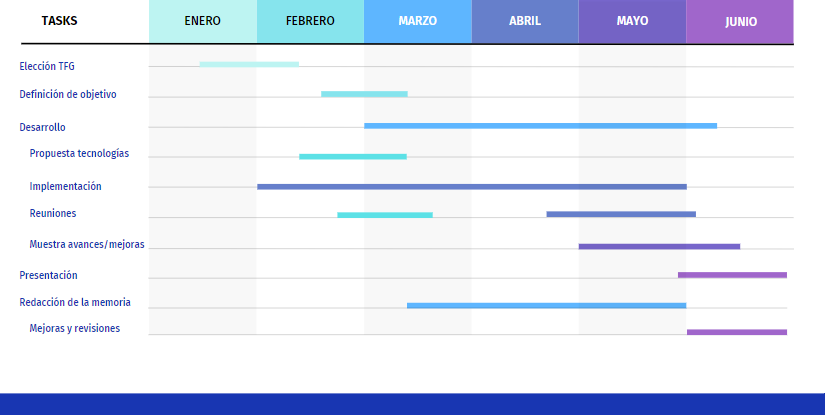
\includegraphics[width=\textwidth]{img/GANTT_TFG.png}
        \caption{Diagrama planificación temporal del proyecto}
        \label{figura:GANTT_TFG}
    \end{figure}
    
%%Lo importante es que quede claro cuánto tiempo has consumido en realizar el TFG/TFM 
%(tiempo natural, p.ej., 6 meses) y a qué nivel de esfuerzo (p.ej., principalmente los 
%fines de semana).


\section{Estructura de la memoria}
\label{sec:estructura}

Por último, en esta sección se introduce a alto nivel la organización del resto del documento
y qué contenidos se van a encontrar en cada capítulo.

    \begin{itemize}
      \item En este primer capítulo se hace una breve introducción al proyecto, se describen los objetivos del mismo y se refleja la planificación temporal.
      \item En el siguiente capítulo se describen las tecnologías implicadas en el desarrollo de este TFG. (Capítulo~\ref{chap:tecnologias}).
      \item En el capítulo~\ref{chap:diseño} Se describe el proceso \textcolor{red}{de desarrollo
      de la herramienta}  \ldots
      \item En el capítulo~\ref{chap:experimentos} Se presentan las principales pruebas realizadas
      para validación de la plataforma/herramienta\ldots (o resultados de los experimentos
      efectuados). Esta sección contiene, con todo detalle, las pruebas realizadas para realizar la comparativa entre herramientas.
      \item Por último, se presentan las conclusiones del proyecto así como los trabajos futuros que podrían derivarse de éste (Capítulo~\ref{chap:conclusiones}).
    \end{itemize}


\section{Github}
\label{sec:planificacion-temporal}
%A continuación, se puede visualizar el cronograma de este Trabajo Fin de Grado.

El código realizado para este Trabajo de Fin de Grado ha sido almacenado en un repositorio de Github. Github es un servicio web que almacena repositorios de proyectos de
desarrollo software que utilizan el sistema de control de versiones Git
%%Lo importante es que quede claro cuánto tiempo has consumido en realizar el TFG/TFM 
%(tiempo natural, p.ej., 6 meses) y a qué nivel de esfuerzo (p.ej., principalmente los 
%fines de semana).

\clearpage

%%%%%%%%%%%%%%%%%%%%%%%%%%%%%%%%%%%%%%%%%%%%%%%%%%%%%%%%%%%%%%%%%%%%%%%%%%%%%%%%
%%%%%%%%%%%%%%%%%%%%%%%%%%%%%%%%%%%%%%%%%%%%%%%%%%%%%%%%%%%%%%%%%%%%%%%%%%%%%%%%
% ESTADO DEL ARTE %
%%%%%%%%%%%%%%%%%%%%%%%%%%%%%%%%%%%%%%%%%%%%%%%%%%%%%%%%%%%%%%%%%%%%%%%%%%%%%%%%

\chapter{Estado del arte}               %% a.k.a "Tecnologías utilizadas"
\label{chap:tecnologias}

Para el desarrollo de este Trabajo Fin de Grado se han utilizado diferentes tecnologías, las cuales se explican en este capítulo.

\section{Atom} 
\label{sec:atom}
Atom\footnote{\url{https://atom.io/}} es un editor de código fuente especializado en la programación. Compatible con los lenguajes más populares, permite escribir código y programar desde tu PC con Windows,Linux o macOS, con soporte para múltiples plug-in escritos en Node.js y control de versiones Git integrado, desarrollado por GitHub. 

La mayor parte de los paquetes tienen licencias de software libre y está desarrollados y mantenidos por la comunidad de usuarios. Atom está basado en Electron (Anteriormente conocido como Atom Shell), un framework que permite crear aplicaciones de escritorio multiplataforma. También puede ser utilizado como un \gls{ide}.

\begin{figure}[H]
        \centering
        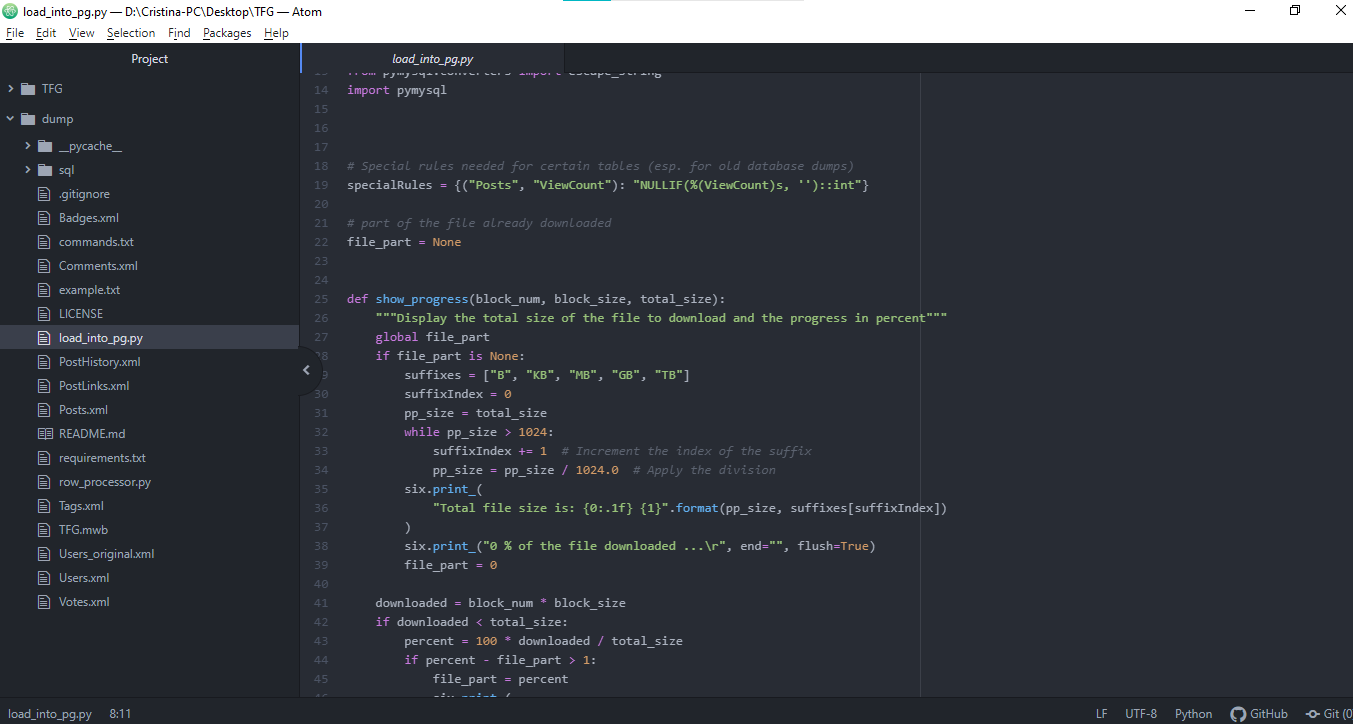
\includegraphics[width=\textwidth]{img/ATOM.png}
        \caption{Interfaz de Atom}
        \label{figura:ATOM}
    \end{figure}

Personalmente, he optado por Atom porque es el editor que suelo utilizar para todos
mis proyectos tanto personales como laborales. 

\section{Python} 
\label{sec:Python}

Python~\cite{van2007python} es un lenguaje de programación interpretado y dinámico, de código abierto, que
soporta tanto el paradigma de la programación orientada a objetos (OOP) como el de la programación funcional.

Se ha elegido este lenguaje de programación para el parseado de datos extraídos de la plataforma de Stack Exchange\footnote{\url{https://stackexchange.com/}}. Además, Python, ofrece múltiples paquetes para la conexión con bases de datos. En este proyecto se ha utilizado el conector oficial de Oracle para MySQL, mysql-connector-python\footnote{\url{https://dev.mysql.com/doc/connector-python/en/connector-python-introduction.html}}, que cumple con la DB API 2.0 de Python~\cite{Python}.

\section{MySQL} 
\label{sec:Mysql}

El sistema gestor de la base de datos elegido para dar soporte a la persistencia de la información y el tratamiento de datos de forma conveniente ha sido MySQL (v8.0)~\cite{MYSQL}.

MySQL es uno de los gestores de base de datos \gls{sql} más popular en la actualidad. Es desarrollado, distribuido y soportado por Oracle. Se trata de un Software de código abierto (OpenSource), que permite que pueda ser modificado dependiendo de las necesidades de cada usuario. El software de MySQL está basado en GPL (GNU General Public License) que define qué y qué no se debe hacer con el software en diferentes situaciones.

MySQL, desde la versión 5.6, proporciona una herramienta denominada  \textit{MySQLWorkbench}~\cite{krogh2020mysql}. Es una herramienta visual de diseño de bases de datos que integra desarrollo de software, administración de bases de datos, diseño de bases de datos, gestión y mantenimiento para el sistema de base de datos MySQL.

Se ha utilizado MySQL ya que es un source nativo tanto en Grafana como en Tableau, además ofrece múltiples ventajas, donde podemos destacar su alto rendimiento, bajo consumo de recursos, soporte a múltiples Sistemas Operativos y una alta securización de los datos.

\section{Tecnologías de visualización y análisis} 
\label{sec:Tenologias_va}
\subsection{Grafana/ Graphite} % título de subsección (se muestra)
\label{sec:Grafana} % identificador de subsección (no se muestra, es para poder referenciarla)

\textbf{Grafana}~\cite{chakraborty2021grafana} es una herramienta de código abierto para la obtención de datos, almacenamiento, visualización y análisis.
Se conecta con todas las fuentes de datos posibles, como \textit{Graphite, Prometheus, Influx DB, ElasticSearch, MySQL, PostgreSQL}, y otros.

Grafana, mediante peticiones SQL en tiempo real a la Base de Datos, representa la
información obtenida en Paneles, que se considera cualquier elemento que represente de forma gráfica la información, y Dashboards, que se trata de una agrupación de paneles, de distinto tipo como, por ejemplo, gráficas de tiempo, sectores cirulares, diagramas de barras, tablas, mapas, etc.


\begin{figure}[H]
        \centering
        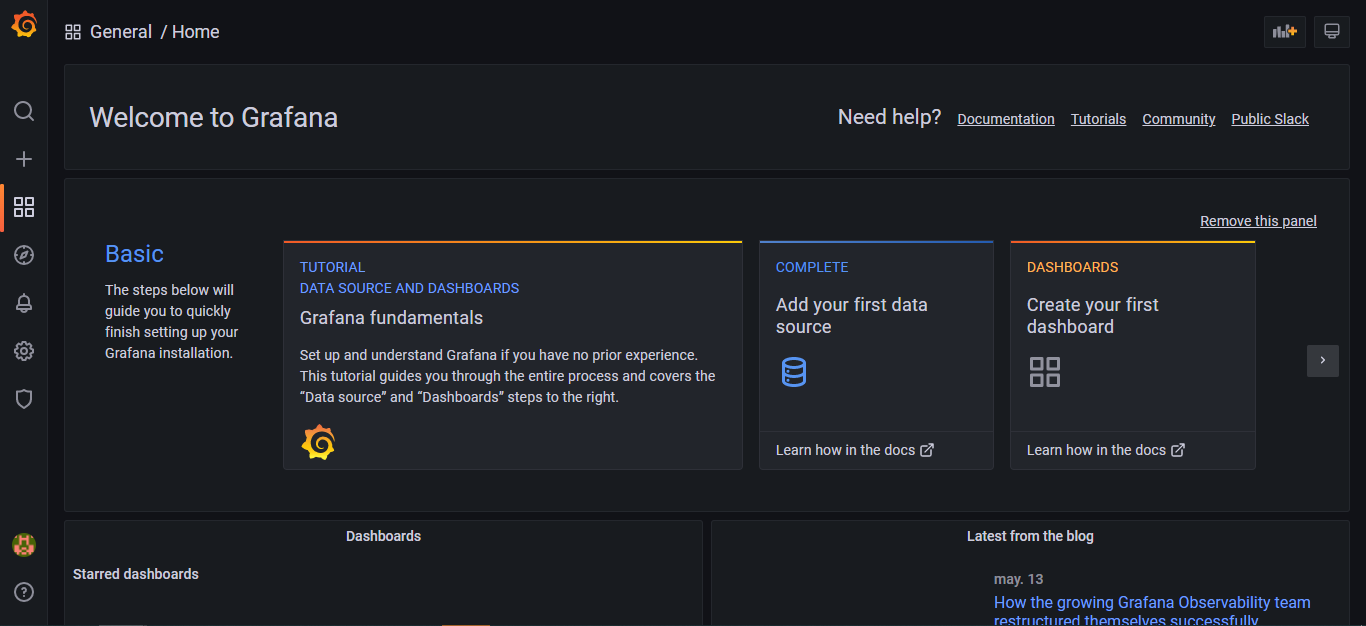
\includegraphics[width=\textwidth]{img/Grafana.png}
        \caption{Interfaz gráfica Grafana}
        \label{figura:Grafana}
    \end{figure}


\textbf{Graphite} ~\cite{Graphite} es una herramienta de monitoreo. Facilita el almacenamiento y visualización de datos de series de tiempo. Idealmente, Graphite se usa como fuente de datos para el tablero de Grafana en una configuración de monitoreo de datos.

Graphite fue diseñado y escrito originalmente por Chris Davis en Orbitz en 2006 como un proyecto paralelo que finalmente se convirtió en su herramienta de monitoreo fundamental. En 2008, Orbitz permitió que Graphite se lanzara bajo la licencia de código abierto Apache 2.0 . Numerosas empresas grandes han implementado Graphite en la producción, donde les ayuda a monitorear sus servicios de comercio electrónico de producción y planificar el crecimiento.

\subsection{Tableau}
\label{sec:tableau}

Tableau~\cite{Tableau} es un software para el análisis y visualización de datos. Tableau se fundó en 2003 como resultado de un proyecto de ciencias de la computación de Stanford. Este tenía como objetivo mejorar el flujo del análisis y poner los datos al alcance de las personas a través de la visualización.  
Tableau destaca por su facilidad para integrar diferentes tipos de datos y permite la creación de dashboards que facilitan  la toma de decisiones a partir de la información generada. Se trata de un programa flexible, ya que puede ser configurado para que trabaje bajo un servidor, en el escritorio o en la nube, visualizando los datos desde el principio. Además, ofrece cientos de conectores nativos para extraer, limpiar y correlacionar fácilmente datos de prácticamente cualquier fuente sin tener que crear un código personalizado.

En este proyecto, se han utilizado dos herramientas que ofrece Tableau: Tableau Prep y Tableau Desktop. El primero, permite transformar y limpiar los datos mediante un proceso totalmente automático. El segundo, es la aplicación principal que lleva a cabo todo el análisis y donde se crean las visualizaciones. 
\begin{figure}[H]
        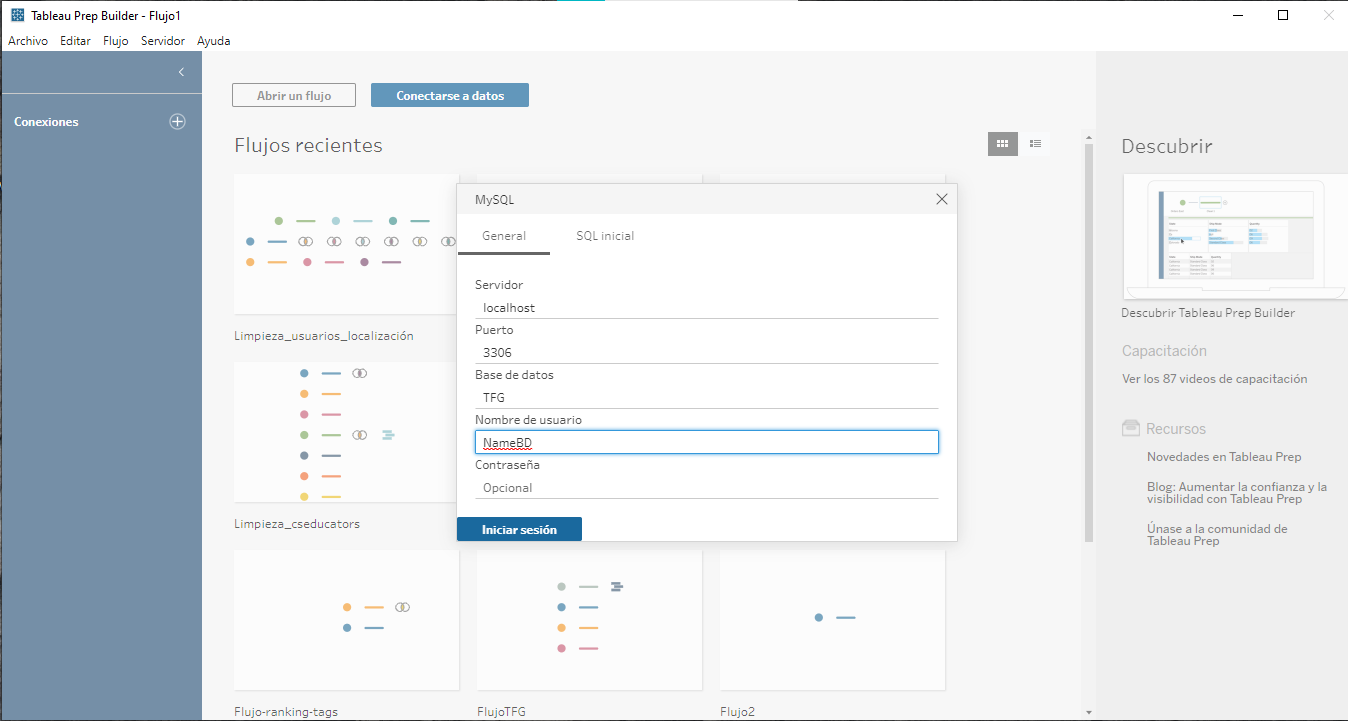
\includegraphics[width=\textwidth]{img/PREP.png}
        \caption{Interfaz gráfica Tableau Prep}
        \label{figura:Grafana}
    \end{figure}
    \begin{figure}[H]
        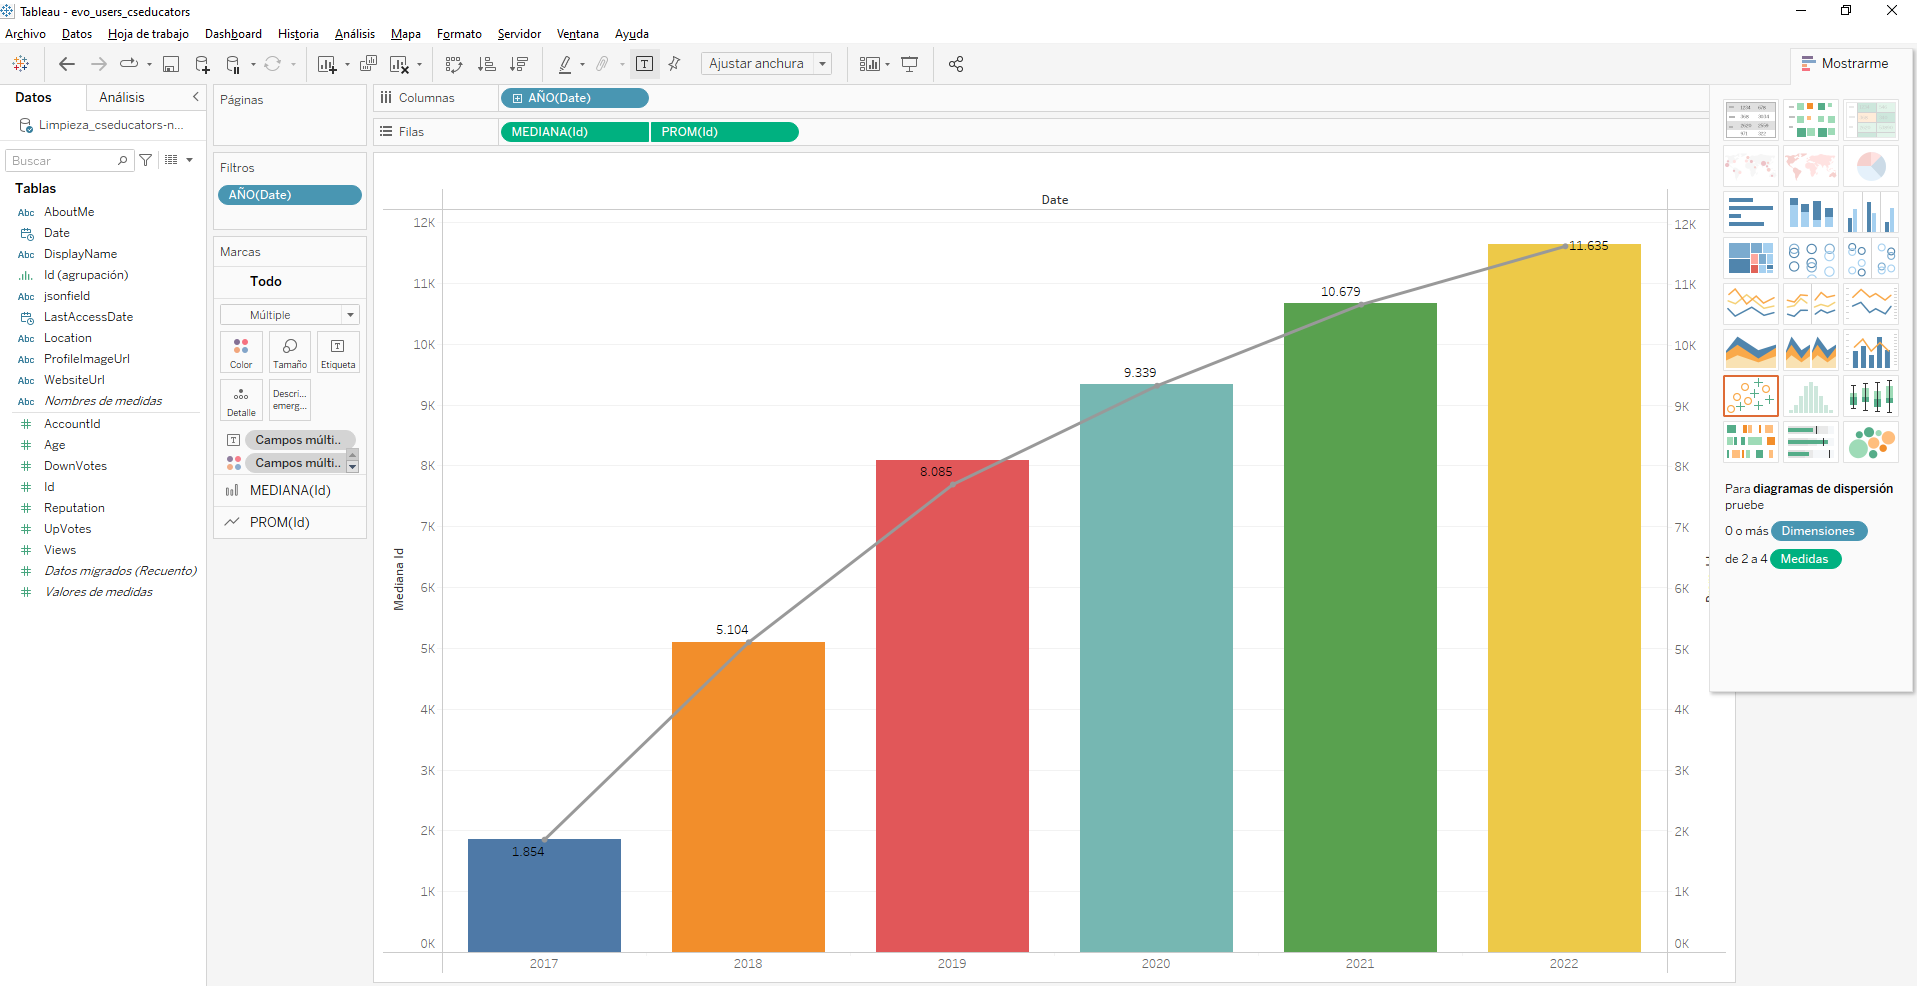
\includegraphics[width=\textwidth]{img/Desktop.png}
        \caption{Interfaz gráfica Tableau Desktop}
        \label{figura:Grafana}
    \end{figure}

    
\section{Comparativa Site by Site}
\label{sec:comparativa}

%%-- El comando \gls{} permite incluir términos en el glosario, para luego reunirlos todos
%%-- en una tabla al comienzo o al final del documento, junto con sus definiciones.

PyCharm es un \gls{ide} dedicado concretamente a la programación en Python y desarrollado por la compañía checa JetBrains.

Proporciona análisis de código, un depurador gráfico, una consola de Python integrada, control de versiones y, además, soporta desarrollo web con Django. Todas estas características lo convierten en un entorno completo e intuitivo, idóneo para el desarrollo de proyectos académicos como el que nos ocupa.

***** METER LOS DATOS DE CRITERIOS DE COMMPARACION (TIPO DE DATOS, Real Time,costes...)



\section{Redacción de la memoria: LaTeX/Overleaf}
\label{sec:redaccion_de_la_memoria}

LaTeX es un sistema de composición tipográfica de alta calidad que incluye características especialmente diseñadas para la producción de documentación técnica y científica. Estas características, entre las que se encuentran la posibilidad de incfluir expresiones matemáticas, fragmentos de código, tablas y referencias, junto con el hecho de que se distribuya como software libre, han hecho que LaTeX se convierta en el estándar de facto para la redacción y publicación de artículos académicos, tesis y todo tipo de documentos científico-técnicos. 

Por su parte, Overleaf es un editor LaTeX colaborativo basado en la nube. Lanzado originalmente en 2012, fue creado por dos matemáticos que se inspiraron en su propia experiencia en el ámbito académico para crear una solución satisfactoria para la escritura científica colaborativa.

Además de por su perfil colaborativo, Overleaf destaca porque, pese a que en LaTeX el escritor utiliza texto plano en lugar de texto formateado (como ocurre en otros procesadores de texto como Microsoft Word, LibreOffice Writer y Apple Pages), éste puede visualizar en todo momento y paralelamente el texto formateado que resulta de la escritura del código fuente.

\cleardoublepage

%%%%%%%%%%%%%%%%%%%%%%%%%%%%%%%%%%%%%%%%%%%%%%%%%%%%%%%%%%%%%%%%%%%%%%%%%%%%%%%%
%%%%%%%%%%%%%%%%%%%%%%%%%%%%%%%%%%%%%%%%%%%%%%%%%%%%%%%%%%%%%%%%%%%%%%%%%%%%%%%%
% DISEÑO E IMPLEMENTACIÓN %
%%%%%%%%%%%%%%%%%%%%%%%%%%%%%%%%%%%%%%%%%%%%%%%%%%%%%%%%%%%%%%%%%%%%%%%%%%%%%%%%

\chapter{Diseño e implementación}
\label{chap:diseño}


Aquí viene todo lo que has hecho tú (tecnológicamente). 
Puedes entrar hasta el detalle. 
Es la parte más importante de la memoria, porque describe lo que has hecho tú.
Eso sí, normalmente aconsejo no poner código, sino diagramas.

\section{Datasets}
\label{sec:datasets}

******* METER LA INFO DEL TIPO DE DATOS, Servidor, parseado.... 
%%-- El comando \gls{} permite incluir términos en el glosario, para luego reunirlos todos
%%-- en una tabla al comienzo o al final del documento, junto con sus definiciones.

PyCharm es un \gls{ide} dedicado concretamente a la programación en Python y desarrollado por la compañía checa JetBrains.

Proporciona análisis de código, un depurador gráfico, una consola de Python integrada, control de versiones y, además, soporta desarrollo web con Django. Todas estas características lo convierten en un entorno completo e intuitivo, idóneo para el desarrollo de proyectos académicos como el que nos ocupa.

\subsection{Parseado de datos}
\label{sec:parser} 
A veces se incluyen nombres de archivos, paquetes, etc. como texto monoespaciado, utilizando
el comando \LaTeX \mintinline{latex}{\texttt{}}. Sin embargo, esto puede generar un problema
cuando las palabras en fuente monoespaciada alcanzan el final de una línea. En ese caso,
el compilador rehusa muchas veces romper la palabra y deja la línea demasiado larga respecto
al resto.

\section{Arquitectura general} 
\label{sec:arquitectura}

Si tu proyecto es un software, siempre es bueno poner la arquitectura (que es cómo se estructura tu programa a ``vista de pájaro'').

Por ejemplo, puedes verlo en la Figura~\ref{fig:arquitectura}.
\LaTeX \ pone las figuras donde mejor cuadran. 
Y eso quiere decir que quizás no lo haga donde lo hemos puesto\ldots
Eso no es malo.
A veces queda un poco raro, pero es la filosofía de \LaTeX: tú al contenido, que yo me encargo de la maquetación.

\begin{figure}
  \centering
  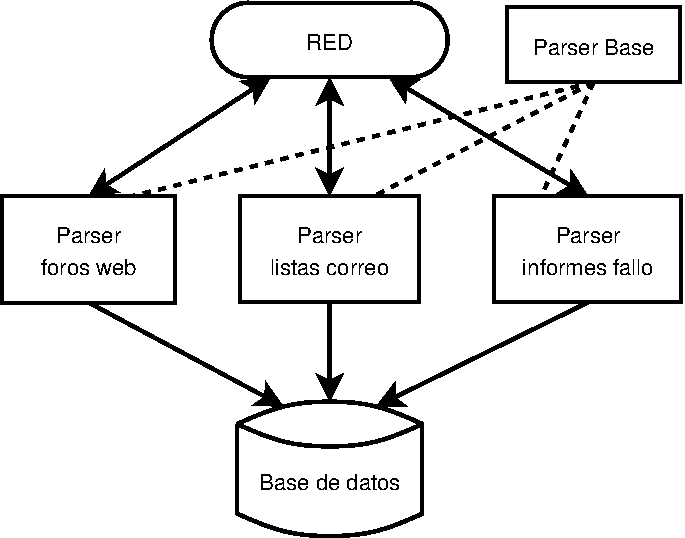
\includegraphics[width=9cm, keepaspectratio]{img/arquitectura.png}
  \caption{Estructura del parser básico.}\label{fig:arquitectura}
\end{figure}

\begin{figure}
    \centering
    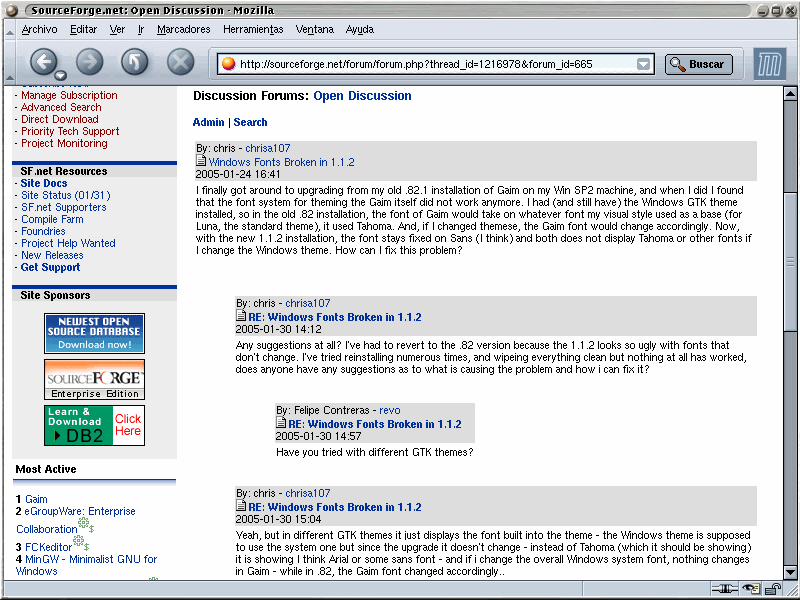
\includegraphics[bb=0 0 800 600, width=12cm, keepaspectratio]{img/foro1}
    \caption{Página con enlaces a hilos}\label{fig:_arquitectura}
\end{figure}

 
Recuerda que toda figura que añadas a tu memoria debe ser explicada.
Sí, aunque te parezca evidente lo que se ve en la Figura~\ref{fig:arquitectura}, la figura en sí solamente es un apoyo a tu texto.
Así que explica lo que se ve en la Figura, haciendo referencia a la misma tal y como ves aquí.
Por ejemplo: En la Figura~\ref{fig:arquitectura} se puede ver que la estructura del \emph{parser} básico, que consta de seis componentes diferentes: los datos se obtienen de la red, y según el tipo de dato, se pasará a un \emph{parser} específico y bla, bla, bla\ldots

Si utilizas una base de datos, no te olvides de incluir también un diagrama de entidad-relación.

\cleardoublepage

%%%%%%%%%%%%%%%%%%%%%%%%%%%%%%%%%%%%%%%%%%%%%%%%%%%%%%%%%%%%%%%%%%%%%%%%%%%%%%%%
%%%%%%%%%%%%%%%%%%%%%%%%%%%%%%%%%%%%%%%%%%%%%%%%%%%%%%%%%%%%%%%%%%%%%%%%%%%%%%%%
% EXPERIMENTOS Y VALIDACIÓN %
%%%%%%%%%%%%%%%%%%%%%%%%%%%%%%%%%%%%%%%%%%%%%%%%%%%%%%%%%%%%%%%%%%%%%%%%%%%%%%%%

\chapter{Experimentos y validación}
\label{chap:experimentos}

\textbf{Atención}: Este capítulo se introdujo como requisito en 2019.

Describe los experimentos y casos de test que tuviste que implementar para validar tus resultados. 
Incluye también los resultados de validación que permiten afirmar que tus resultados son correctos.

\section{Experimento Stack Exchange}
\label{chap:exper_stack}

Es bastante habitual que se reproduzcan fragmentos de código en la memoria de un TFG/TFM.
Esto permite explicar detalladamente partes del desarrollo que se ha realizado que se consideren
de especial interés. No obstante, tampoco es conveniente pasarse e incluir demasiado código en
la memoria, puesto que se puede alargar mucho el documento. Un recurso muy habitual es subir
todo el código a un repositorio de un servicio de control de versiones como GitHub o GitLab,
y luego incluir en la memoria la URL que enlace a dicho repositorio.

Para incluir fragmentos de código en un documento \LaTeX se pueden combinar varias
herramientas:

\subsection{Localización}
\section{Incorporación de código en la memoria}

Es bastante habitual que se reproduzcan fragmentos de código en la memoria de un TFG/TFM.
Esto permite explicar detalladamente partes del desarrollo que se ha realizado que se consideren
de especial interés. No obstante, tampoco es conveniente pasarse e incluir demasiado código en
la memoria, puesto que se puede alargar mucho el documento. Un recurso muy habitual es subir
todo el código a un repositorio de un servicio de control de versiones como GitHub o GitLab,
y luego incluir en la memoria la URL que enlace a dicho repositorio.

Para incluir fragmentos de código en un documento \LaTeX se pueden combinar varias
herramientas:

\begin{itemize}
    \item El entorno \mintinline{latex}{\begin{listing}[]...\end{listing}} permite crear
    un marco en el que situar el fragmento de código (parecido al generado cuando insertamos
    una tabla o una figura). Podemos insertar también una descripción (\textit{caption})
    y una etiqueta para referenciarlo luego en el texto.
    
    \item Dentro de este entorno, se puede utilizar el paquete 
    \mintinline{latex}{minted}~\footnote{\url{https://es.overleaf.com/learn/latex/Code_Highlighting_with_minted}},
    que utiliza el paquete Python Pygments para resaltado de sintaxis (coloreando el
    código). Como se puede ver en el siguiente ejemplo, hay muchas opciones de configuración
    que permiten controlar cómo se va a mostrar el código (incluir números de línea, saltos
    de línea, tamaño y tipo de fuente, espaciado, código de colores para resaltado, etc.).
\end{itemize}

\begin{listing}[h!]
    \caption{Lectura de un fichero *.csv y tipado de datos.}{}
    \label{lst:1}
    \begin{minted}[breaklines, fontsize=\footnotesize, baselinestretch=1]{python}
# A dictionary is built to define the data type contained by each column
dtype_scheme ={'budget': np.int64, 'genres': np.object, 'homepage': np.str, 'id': np.int64, 'keywords': np.object, 'original_language': np.str, 'original_title': np.str, 'overview': np.str, 'popularity': np.float64, 'production_companies': np.object, 'production_countries': np.object, 'release_date': np.object, 'revenue': np.int64, 'runtime': np.float64, 'spoken_languages': np.object,  'status': np.object, 'tagline': np.str, 'title': np.str, 'vote_average': np.float64, 'vote_count': np.int64}

# When loading the data from the .csv file, we provide the scheme to be followed for data typing
df1 = dd.read_csv('tmdb_5000_movies.csv', dtype=dtype_scheme)
    \end{minted}
\end{listing}

Otra ventaja del entorno \verb|listing| es que se puede generar automáticamente un índice
(con entradas hiperenlazadas) de fragmentos de código, para incluirlo al comienzo del 
documento junto con los índices de figuras, tablas, etc.

\subsection{Fuentes monoespaciadas}

A veces se incluyen nombres de archivos, paquetes, etc. como texto monoespaciado, utilizando
el comando \LaTeX \mintinline{latex}{\texttt{}}. Sin embargo, esto puede generar un problema
cuando las palabras en fuente monoespaciada alcanzan el final de una línea. En ese caso,
el compilador rehusa muchas veces romper la palabra y deja la línea demasiado larga respecto
al resto.

Para evitar esto, especialmente en párrafos más cortos de lo habitual (como en una lista
no numerada), se puede utilizar el comando \mintinline{latex}{\begin{sloppypar}...\end{sloppypar}},
como se muestra a continuación con un ejemplo real.
    
\begin{itemize}
    
    \begin{sloppypar} % Arregla longitud de línea en párrafos con fuente monoespaciada
    \item Los valores contenidos en las columnas \texttt{genres}, \texttt{spoken\_languages}, \texttt{production\_companies} y \texttt{production\_countries}, clasificados originalmente como \texttt{np.objects}, se corresponden en realidad con listas de objetos \gls{json} que han sido almacenadas como cadenas de caracteres. A través de la función \texttt{get\_values(obj, key)} definida específicamente para ello, se transformará dicha cadena de caracteres en una lista de diccionarios a través de la función \texttt{json.loads(obj)} y se devolverá una  tupla que recopile los valores de los mismos para la clave indicada, un objeto de Python mucho más manejable de cara a realizar consultas sobre el \textit{dataset}.
    \end{sloppypar}
    
\end{itemize}

\cleardoublepage

%%%%%%%%%%%%%%%%%%%%%%%%%%%%%%%%%%%%%%%%%%%%%%%%%%%%%%%%%%%%%%%%%%%%%%%%%%%%%%%%
%%%%%%%%%%%%%%%%%%%%%%%%%%%%%%%%%%%%%%%%%%%%%%%%%%%%%%%%%%%%%%%%%%%%%%%%%%%%%%%%
% CONCLUSIONES %
%%%%%%%%%%%%%%%%%%%%%%%%%%%%%%%%%%%%%%%%%%%%%%%%%%%%%%%%%%%%%%%%%%%%%%%%%%%%%%%%


\chapter{Conclusiones y trabajos futuros}
\label{chap:conclusiones}


\section{Consecución de objetivos}
\label{sec:consecucion-objetivos}

Esta sección es la sección espejo de las dos primeras del capítulo de objetivos, donde se planteaba el objetivo general y se elaboraban los específicos.

Es aquí donde hay que debatir qué se ha conseguido y qué no. 
Cuando algo no se ha conseguido, se ha de justificar, en términos de qué problemas se han encontrado y qué medidas se han tomado para mitigar esos problemas.

Y si has llegado hasta aquí, siempre es bueno pasarle el corrector ortográfico, que las erratas quedan fatal en la memoria final.
Para eso, en Linux tenemos aspell, que se ejecuta de la siguiente manera desde la línea de \emph{shell}:

\begin{minted}{bash}
  aspell --lang=es_ES -c memoria.tex
\end{minted}

\section{Aplicación de lo aprendido}
\label{sec:aplicacion}

Aquí viene lo que has aprendido durante el Grado/Máster y que has aplicado en el TFG/TFM. Una buena idea es poner las asignaturas más relacionadas y comentar en un párrafo los conocimientos y habilidades puestos en práctica.

\begin{enumerate}
  \item a
  \item b
\end{enumerate}


\section{Lecciones aprendidas}
\label{sec:lecciones_aprendidas}

Aquí viene lo que has aprendido en el Trabajo Fin de Grado/Máster.

\begin{enumerate}
  \item Aquí viene uno.
  \item Aquí viene otro.
\end{enumerate}


\section{Trabajos futuros}
\label{sec:trabajos_futuros}

Ningún proyecto ni software se termina, así que aquí vienen ideas y funcionalidades que estaría bien tener implementadas en el futuro.

Es un apartado que sirve para dar ideas de cara a futuros TFGs/TFMs.


%%%%%%%%%%%%%%%%%%%%%%%%%%%%%%%%%%%%%%%%%%%%%%%%%%%%%%%%%%%%%%%%%%%%%%%%%%%%%%%%
%%%%%%%%%%%%%%%%%%%%%%%%%%%%%%%%%%%%%%%%%%%%%%%%%%%%%%%%%%%%%%%%%%%%%%%%%%%%%%%%
% GLOSARIO(S) %
%%%%%%%%%%%%%%%%%%%%%%%%%%%%%%%%%%%%%%%%%%%%%%%%%%%%%%%%%%%%%%%%%%%%%%%%%%%%%%%%
\glsaddall
\printglossary[type=\acronymtype]

\printglossary

%%%%%%%%%%%%%%%%%%%%%%%%%%%%%%%%%%%%%%%%%%%%%%%%%%%%%%%%%%%%%%%%%%%%%%%%%%%%%%%%
%%%%%%%%%%%%%%%%%%%%%%%%%%%%%%%%%%%%%%%%%%%%%%%%%%%%%%%%%%%%%%%%%%%%%%%%%%%%%%%%
% APÉNDICE(S) %
%%%%%%%%%%%%%%%%%%%%%%%%%%%%%%%%%%%%%%%%%%%%%%%%%%%%%%%%%%%%%%%%%%%%%%%%%%%%%%%%

%\cleardoublepage
%\appendix
%\chapter{Manual de usuario}
%\label{app:manual}


%%%%%%%%%%%%%%%%%%%%%%%%%%%%%%%%%%%%%%%%%%%%%%%%%%%%%%%%%%%%%%%%%%%%%%%%%%%%%%%%
%%%%%%%%%%%%%%%%%%%%%%%%%%%%%%%%%%%%%%%%%%%%%%%%%%%%%%%%%%%%%%%%%%%%%%%%%%%%%%%%
% BIBLIOGRAFIA %
%%%%%%%%%%%%%%%%%%%%%%%%%%%%%%%%%%%%%%%%%%%%%%%%%%%%%%%%%%%%%%%%%%%%%%%%%%%%%%%%

\cleardoublepage


% https://www.overleaf.com/learn/latex/Bibliography_management_with_biblatex
\raggedright\printbibliography[heading=bibintoc,title={Referencias}]

\end{document}
